\begin{figure}
	\centering
	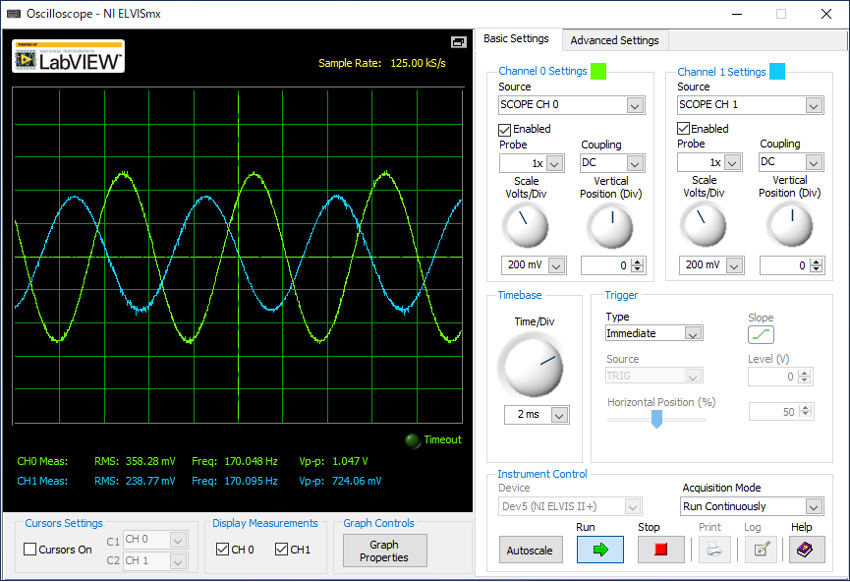
\includegraphics[width=0.8\linewidth]{src/figures/exp8/low-pass.png}
	\caption{ローパスフィルターのカットオフ周波数における波形}\label{fig:exp8-raw-cutoff}
\end{figure}

\begin{figure}
	\centering
	\begin{subfigure}{0.8\linewidth}
		\centering
		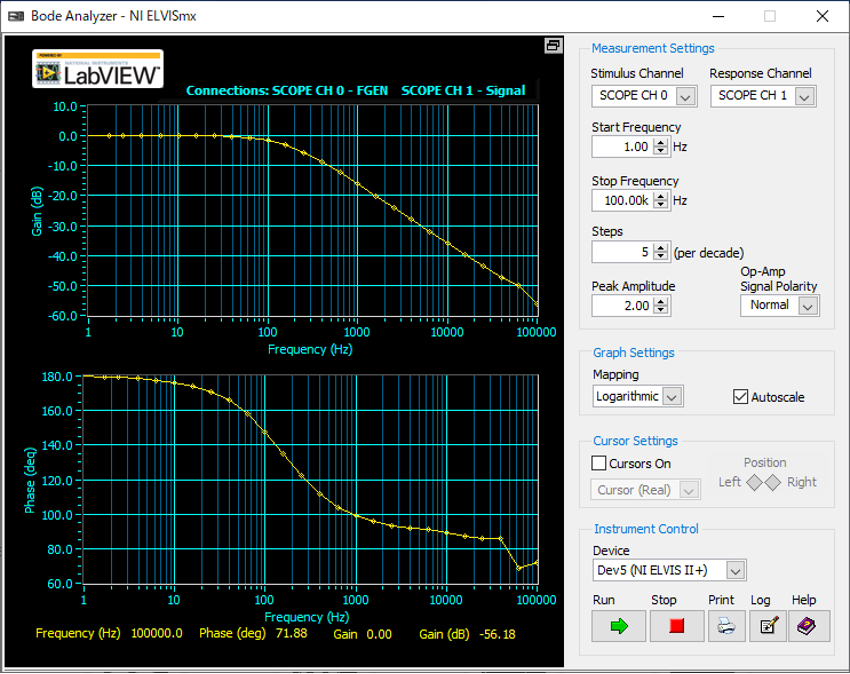
\includegraphics[width=0.8\linewidth]{src/figures/exp8/low-pass-bode-10k.png}
		\subcaption{$R_1=\SI{10}{k\ohm}$}
	\end{subfigure}
	\begin{subfigure}{0.8\linewidth}
		\centering
		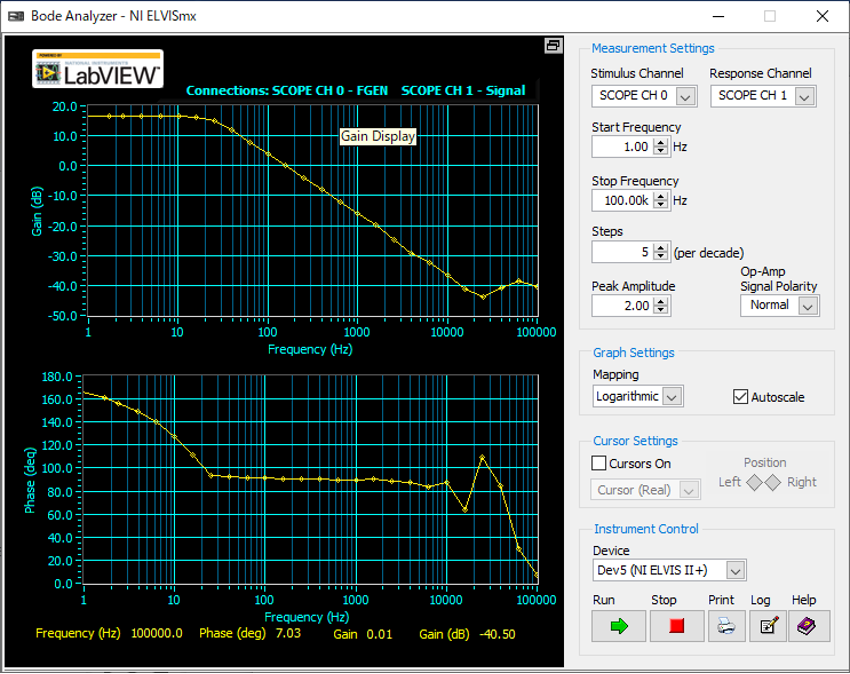
\includegraphics[width=0.8\linewidth]{src/figures/exp8/low-pass-bode-1m.png}
		\subcaption{$R_1=\SI{1}{M\ohm}$}
	\end{subfigure}
	\caption{ローパスフィルターのボード線図}\label{fig:exp8-bode}
\end{figure}
